\chapter{Startup Foundation with Gitea}
\ChapterLabel{Gitea}
\index{Gitea}
\index{startup DevSecOps process}

\section{Overview and Status}
This chapter answers the course manual's Chapter~2 \cite{DosManual}: the
startup's Gitea work hub with a student domain, HTTPS, minimal public
exposure, and persistent data. The eight numbered subsections below match the
eight rubric rows (100 points) in the same order. Optional backup and restore
evidence is a separate extra-credit subsection and is not part of the eight; it is optional and has no owner; the group will decide later whether time allows it.

\begin{devopsNote}[Provider status]
The assignment specifies a DigitalOcean Droplet. Group~1 asked the instructor
whether AWS could be used instead. On October 12, 2026 (8:36\,pm, Canvas
message ``Gitea Assignment --- Question on Cloud Provider (Group 1)'') the
instructor replied that any hosting service is allowed, including AWS or the
group's own servers, \textbf{as long as they are available online and can be
used by the TA and the instructor to test the assignments.} Group~1 therefore
uses AWS. The deployment must stay reachable and testable by the TA and
instructor until grading is complete.
\end{devopsNote}

\begin{tabularx}{\linewidth}{L{5.2cm}L{1.4cm}L{1.6cm}Y}
\caption{Rubric rows, owners, and status\label{Table:GiteaStatus}}\\
\toprule \textbf{Subsection} & \textbf{Points} & \textbf{Owner} & \textbf{Status}\\ \midrule
\endfirsthead
\toprule \textbf{Subsection} & \textbf{Points} & \textbf{Owner} & \textbf{Status}\\ \midrule
\endhead \bottomrule \endlastfoot
Student Pack domain and DNS & 10 & BD & \StatusPending\\
Pinned Gitea deployment & 10 & BD & \StatusPending\\
Database and persistence & 10 & SD & \StatusPending\\
HTTPS and certificate renewal & 15 & BD & \StatusPending\\
Firewall and external exposure & 15 & BD & \StatusPending\\
Startup team workflow & 20 & SD & \StatusPending\\
Architecture and operation & 5 & SD & \StatusPending\\
Manual quality and controls & 15 & SD & \StatusPending\\
Extra credit: backup and restore (optional) & up to 20 & unassigned & \StatusPending\\
\end{tabularx}

\section{Required Subsections}
% ======================================================================
% Region: giteaDomainDns (single owner; edit only your own region)
\subsection{Student Pack domain and DNS (10 points)}
\label{Section:giteaDomainDns}
\index{Gitea!student pack domain and dns}
\textbf{Owner:} BD. Domain registration: \StatusPass{} (order confirmed, \$0.00). Stored card removed: \StatusPass{}. DNS record and public-resolver lookup: \StatusPass{}. Teammate lookup and HTTPS link: \StatusPending{}.

\paragraph{Offer and eligibility.}
The domain comes from the GitHub Student Developer Pack, which lists domain
offers from Namecheap, Name.com, and .TECH Domains \cite{GitHubPackDomains}.
The group's Student Pack is approved on Brahmi Dalvi's GitHub account. The
Namecheap offer was started first but its GitHub authorization page requested
the \texttt{repo} scope (read and write access to all public and private
repositories), which the group judged too broad for a domain claim, so it was
cancelled. The Name.com Education Pack authorization requested ``public data
only'' and was accepted.

\paragraph{Domain and costs.}
\begin{tabularx}{\linewidth}{L{4.2cm}Y}
\caption{Domain registration facts\label{Table:DomainFacts}}\\
\toprule \textbf{Item} & \textbf{Value}\\ \midrule
\endfirsthead
\toprule \textbf{Item} & \textbf{Value}\\ \midrule
\endhead \bottomrule \endlastfoot
Domain & \texttt{ssw590-g1.tech}, registered at Name.com, order \#28974415. The confirmation email arrived Thursday, October 15, 2026 at 00:36 (mailbox local time) and gives the order date as October 14, 2026; the one-day difference is consistent with Name.com stamping the date in a different time zone, which we did not confirm\\
Planned Gitea hostname & \texttt{\GiteaHost} (A record created, see below)\\
First-year cost & \$0.00 (cart total \$0.00; the regular price shown struck through in the cart was \$89.99)\\
Renewal cost & \$89.99 (``Renew for \$89.99'' on the domain page)\\
Expiration & October 15, 2027\\
Automatic renewal & OFF (turned off after registration)\\
Extras declined & Domain Safe Pro (\$7.99/year); the free Domain Safe plan (domain lock, WHOIS privacy, free SSL certificate) is included\\
\end{tabularx}
The order summary after checkout also shows a struck-through \$7.99 next to the
domain; the group did not investigate that figure and relies on the \$0.00
total and the \$89.99 renewal price shown on the domain page.
Figure~\ref{Fig:DomainOrder} shows the completed order and
Figure~\ref{Fig:DomainDetails} shows the domain page after automatic renewal
was turned off.

\begin{figure}[htbp]
\centering
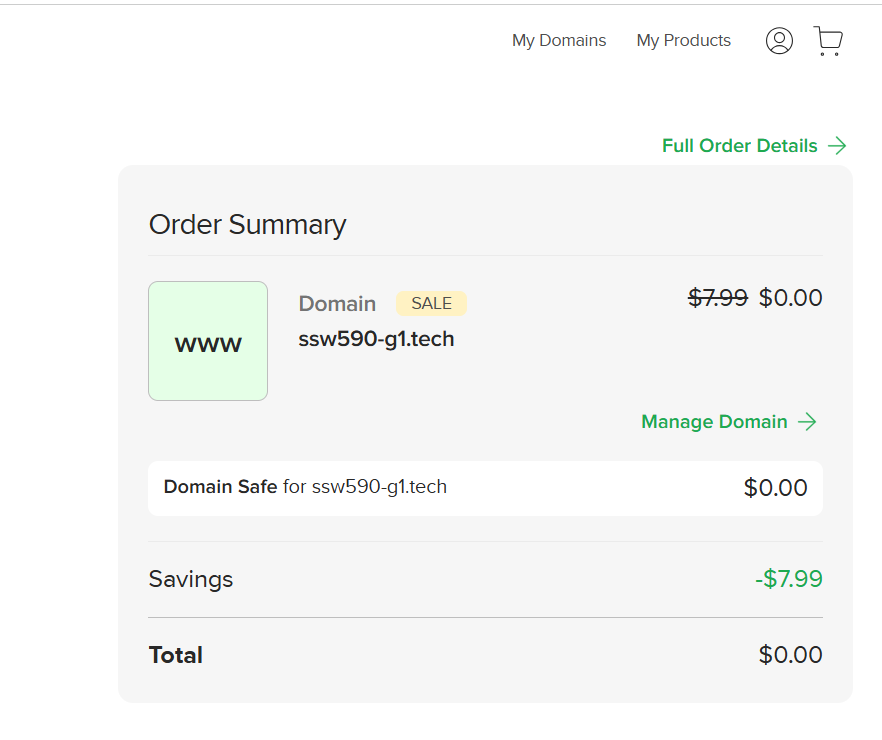
\includegraphics[width=0.7\linewidth]{../evidence/02-namecom-order-summary-ssw590-g1-tech-total-0.00-2026-10-15.png}
\caption{Name.com order summary, October 15, 2026: domain and free Domain Safe, total \$0.00.}
\label{Fig:DomainOrder}
\end{figure}

\begin{figure}[htbp]
\centering
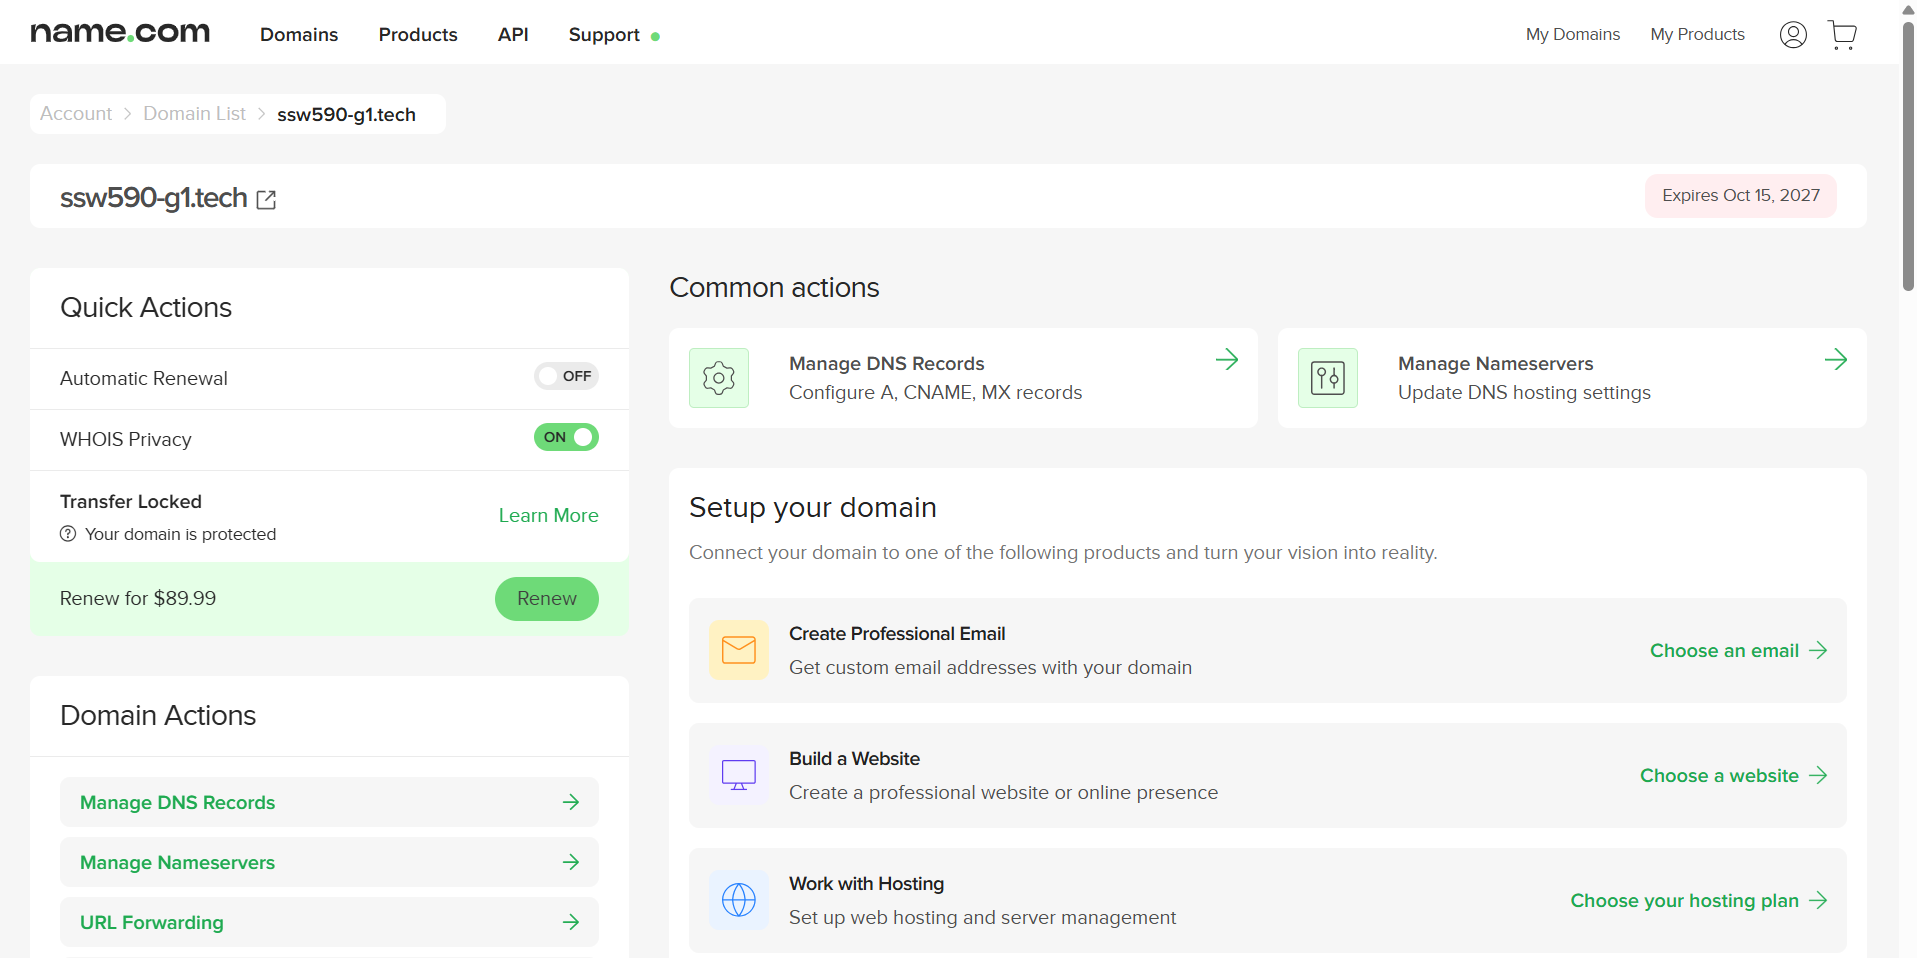
\includegraphics[width=\linewidth]{../evidence/04-namecom-domain-details-expires-2027-10-15-autorenew-OFF-2026-10-15.png}
\caption{Domain page, October 15, 2026: expires October 15, 2027, automatic renewal OFF, renewal price \$89.99.}
\label{Fig:DomainDetails}
\end{figure}

\paragraph{Renewal tracking.}
The group does not plan to renew: the domain is needed only through grading,
and the TA and instructor must be able to reach the service until then. Expiry
is October 15, 2027. \Todo{name the owner and calendar reminder for this date}

\paragraph{DNS record.}
In Name.com's DNS manager the group created one record, \texttt{A git.ssw590-g1.tech
52.73.254.36} with TTL 300 (Figure~\ref{Fig:DnsRecord}). The address is the Elastic
IP of the EC2 instance described in the deployment subsection. No AAAA record was
created, because the deployment is IPv4 only. The domain uses Name.com's own
nameservers (\texttt{ns1bqx}, \texttt{ns2kry}, \texttt{ns3jmt}, \texttt{ns4ksy}
\texttt{.name.com}).

\begin{figure}[htbp]
\centering
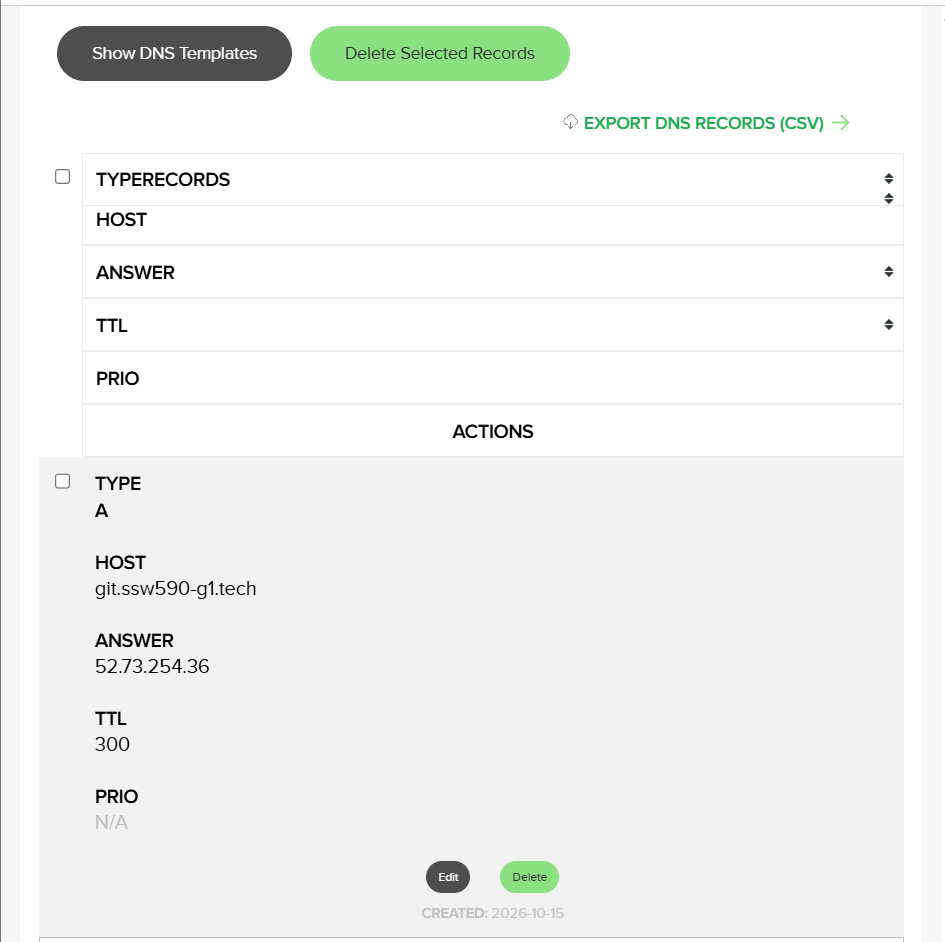
\includegraphics[width=0.6\linewidth]{../evidence/10-namecom-dns-a-record-git-ssw590-g1-tech-2026-10-15.png}
\caption{Name.com DNS records for \texttt{ssw590-g1.tech}, October 15, 2026: one A record for \texttt{git}.}
\label{Fig:DnsRecord}
\end{figure}

\paragraph{Lookup result.}
At 17:30:34 UTC on October 15, 2026 the name resolved to the expected address
through three public resolvers (expected: \texttt{52.73.254.36}; actual: the same).
\begin{center}
\begin{tabular}{lll}
\toprule \textbf{Resolver} & \textbf{Result for \texttt{\GiteaHost}} & \textbf{TTL}\\ \midrule
8.8.8.8 (Google) & A 52.73.254.36 & 300\\
1.1.1.1 (Cloudflare) & A 52.73.254.36 & 300\\
9.9.9.9 (Quad9) & A 52.73.254.36 & 300\\ \bottomrule
\end{tabular}
\end{center}
These lookups were run from Brahmi Dalvi's computer through public resolvers; they
were not run by a teammate on a separate network, so the independent-lookup
wording of the assignment is met only in that sense.
\Todo{optional: a teammate repeats the lookup (for example \texttt{nslookup \GiteaHost{} 8.8.8.8}) from another network and the result is added}.
The HTTPS hostname link will resolve once Gitea and the proxy are deployed.
\Todo{add the clickable HTTPS link once the site is live}

\paragraph{Payment safeguards.}
Name.com required a card even for the \$0.00 order. To avoid an unintended
renewal charge, the group turned automatic renewal off and deleted the stored
payment profile; the billing page then reads ``No saved payment profiles''
(evidence file \texttt{05-namecom-billing-no-saved-payment-profiles-2026-10-15.png}).
The confirmation email shows order \#28974415 with an order total of \$0.00
(evidence file \texttt{06-namecom-order-confirmed-email-order-28974415-received-2026-10-15-0036.png}). \Todo{after a few days, check the card statement and record whether any charge appeared}

% ======================================================================
% Region: giteaDeployment (single owner; edit only your own region)
\subsection{Pinned Gitea deployment (10 points)}
\label{Section:giteaDeployment}
\index{Gitea!pinned gitea deployment}
\textbf{Owner:} BD. \StatusPending{} No evidence recorded yet.

\textbf{Required content (from the course manual):}
\begin{itemize}[nosep]
  \item Droplet/EC2 and Gitea image versions, image source (Docker Hub \texttt{gitea/gitea})
  \item Deployment commands, restart policy, persistent mounts, proxy connection
  \item Redacted Compose excerpt and link to \texttt{gitea/docker-compose.yml} in the team repository
  \item Steps another team could repeat
\end{itemize}

\Todo{write the explanation, then add dated, labeled, sanitized evidence (expected vs.\ actual). A screenshot alone does not replace an explanation. Never claim a test that was not run.}

% ======================================================================
% Region: giteaDatabase (single owner; edit only your own region)
\subsection{Database and persistence (10 points)}
\label{Section:giteaDatabase}
\index{Gitea!database and persistence}
\textbf{Owner:} SD. \StatusPending{} No evidence recorded yet.

\textbf{Required content (from the course manual):}
\begin{itemize}[nosep]
  \item \textbf{Decision (final, team, October 12, 2026): SQLite.} Record the settings, the database-file path under the persistent \texttt{/data} volume, the volume mount, and why no database secret exists. Justify: two-person team, no extra container or credential, simple consistent backup; note it may not suit higher concurrency
  \item Repository and issue identifiers created before the test
  \item Exact container-replacement command (volumes kept), before/after evidence, conclusion
  \item Not applicable: PostgreSQL is not used, so there is no database port, healthcheck, or database secret to document
\end{itemize}

\Todo{write the explanation, then add dated, labeled, sanitized evidence (expected vs.\ actual). A screenshot alone does not replace an explanation. Never claim a test that was not run.}

% ======================================================================
% Region: giteaHttps (single owner; edit only your own region)
\subsection{HTTPS and certificate renewal (15 points)}
\label{Section:giteaHttps}
\index{Gitea!https and certificate renewal}
\textbf{Owner:} BD. \StatusPending{} No evidence recorded yet.

\textbf{Required content (from the course manual):}
\begin{itemize}[nosep]
  \item Comparison of two certificate options and the justification for the chosen one
  \item Where TLS terminates; how private traffic reaches Gitea
  \item Valid hostname certificate: issuer and expiry
  \item HTTP-to-HTTPS redirect behaviour
  \item Renewal automation plus a successful renewal test or dry run
  \item Redacted proxy configuration and test output
\end{itemize}

\Todo{write the explanation, then add dated, labeled, sanitized evidence (expected vs.\ actual). A screenshot alone does not replace an explanation. Never claim a test that was not run.}

% ======================================================================
% Region: giteaFirewall (single owner; edit only your own region)
\subsection{Firewall and external exposure (15 points)}
\label{Section:giteaFirewall}
\index{Gitea!firewall and external exposure}
\textbf{Owner:} BD. \StatusPending{} No evidence recorded yet.

\textbf{Required content (from the course manual):}
\begin{itemize}[nosep]
  \item Cloud firewall / security group name and attachment, inbound rules, source ranges, IPv4 and IPv6
  \item Host and Compose port mappings
  \item Small network diagram
  \item External test (source, time, expected vs.\ actual) for 443, 80, admin SSH, Gitea backend 3000, database port
  \item Corrections made; why HTTPS does not replace a firewall
\end{itemize}

\Todo{write the explanation, then add dated, labeled, sanitized evidence (expected vs.\ actual). A screenshot alone does not replace an explanation. Never claim a test that was not run.}

% ======================================================================
% Region: giteaWorkflow (single owner; edit only your own region)
\subsection{Startup team workflow (20 points)}
\label{Section:giteaWorkflow}
\index{Gitea!startup team workflow}
\textbf{Owner:} SD. \StatusPending{} No evidence recorded yet.

\textbf{Required content (from the course manual):}
\begin{itemize}[nosep]
  \item Links to the organization and product repository; README
  \item Two members and their roles
  \item At least five actionable issues (product and operations)
  \item Two issues traced through linked branch/PR, peer review, merge, closure (needs both members)
\end{itemize}

\Todo{write the explanation, then add dated, labeled, sanitized evidence (expected vs.\ actual). A screenshot alone does not replace an explanation. Never claim a test that was not run.}

% ======================================================================
% Region: giteaArchitecture (single owner; edit only your own region)
\subsection{Architecture and operation (5 points)}
\label{Section:giteaArchitecture}
\index{Gitea!architecture and operation}
\textbf{Owner:} SD. \StatusPending{} No evidence recorded yet.

\textbf{Required content (from the course manual):}
\begin{itemize}[nosep]
  \item Architecture diagram: end-to-end request and data paths
  \item Where data lives; which interfaces are public vs.\ private
  \item How the team restarts and troubleshoots the service
  \item Persistence test is not a backup/restore test
\end{itemize}

\Todo{write the explanation, then add dated, labeled, sanitized evidence (expected vs.\ actual). A screenshot alone does not replace an explanation. Never claim a test that was not run.}

% ======================================================================
% Region: giteaManualQuality (single owner; edit only your own region)
\subsection{Manual quality and controls (15 points)}
\label{Section:giteaManualQuality}
\index{Gitea!manual quality and controls}
\textbf{Owner:} SD. \StatusPending{} No evidence recorded yet.

\textbf{Required content (from the course manual):}
\begin{itemize}[nosep]
  \item Increase the manual version; dated history entries for initial setup and this update, linking sections and evidence
  \item Update Hosts and Passwords tables (hints only) and mention both in the history
  \item Headings, captions, citations, glossary/index entries; secrets redacted
  \item State any failed tests and corrective actions
\end{itemize}

\Todo{write the explanation, then add dated, labeled, sanitized evidence (expected vs.\ actual). A screenshot alone does not replace an explanation. Never claim a test that was not run.}


\section{Extra Credit}
% ======================================================================
% Region: giteaExtraCredit (single owner; edit only your own region)
\subsection{Extra credit: verified backup and restore (up to 20 extra-credit points; optional, unassigned)}
\label{Section:giteaExtraCredit}
\index{Gitea!optional extra credit: verified backup and restore}
\textbf{Owner:} unassigned (decided later if time allows). \StatusPending{} No evidence recorded yet.

\textbf{Required content (from the course manual):}
\begin{itemize}[nosep]
  \item Backup method, coverage, storage location, time (5)
  \item Sanitized backup log/listing; DB and app data form one recoverable state (5)
  \item Test repository and issue present and usable in a separate temporary restored instance, with restore log and screenshots (10)
  \item Do not overwrite the working service; do not include archives, dumps, or keys
\end{itemize}

\Todo{write the explanation, then add dated, labeled, sanitized evidence (expected vs.\ actual). A screenshot alone does not replace an explanation. Never claim a test that was not run.}

